
\section{Experiments} \label{sec:exp}

ToDo by Jan

{\LowerUnits} has been implemented as a prototype\footnote{Source code available at \url{https://github.com/jgorzny/Skeptik}} in the functional programming language Scala\footnote{\url{http://www.scala-lang.org/}} as part of the \skeptik
 library\footnote{\url{https://github.com/Paradoxika/Skeptik}}. {\LowerUnits} has been implemented as a
 recursive \FuncSty{delete} improvement.

%number to change - Jan
The algorithm has been applied to {\bf 308} proofs produced by the {\SPASS}\footnote{\url{http://www.verit-solver.org/}} theorem prover on unsatisfiable benchmarks from the TPTP Problem Library\footnote{\url{http://www.cs.miami.edu/~tptp/}}. The proofs used were restricted to those which could be solved within 300 seconds by {\SPASS} on the Euler Cluster at the University of Victoria\footnote{\url{https://rcf.uvic.ca/euler.php}} using only the contraction and unifying resolution inference rules.

For each proof $\psi$ (with the result of {\LowerUnits} applied to the proof denoted by $\alpha(\psi)$), the time to compress the proof ($t(\psi)$), the compression ratio ($(|\psi|-|\alpha(\psi)|)/|\psi|$), the resolution compression ratio  ($(|\psi|_R-|\alpha(\psi)|_R)/|\psi|_R$), the compression speed ($(|\psi|-|\alpha(\psi)|)/t(\psi)$), and resolution compression speed ($(|\psi|_R-|\alpha(\psi)|_R)/t(\psi)$) were measured\footnote{The raw data is available at \url{https://docs.google.com/spreadsheets/d/1F1-t2OuhypmTQhLU6yTj42aiZ5CqqaZvhVvOzeFgn0k/edit\#gid=1182923972}}, where $|\psi|_R$ indicates the number of resolution inference rules in the proof $\psi$.


The experiments were executed on a laptop (2.8GHz Intel Core i7 processor with 4 GB of RAM (1333MHz DDR3) available to the Java Virtual Machine), and the prototype implementation performed well on this system. Figure \ref{} shows the compression time $t(\psi)$ for each proof, sorted by proof length, and figure \ref{} (respectively figure \ref{}) shows the compression speed (respectively resolution compression speed) for each proof, also sorted by proof length.

\begin{figure}
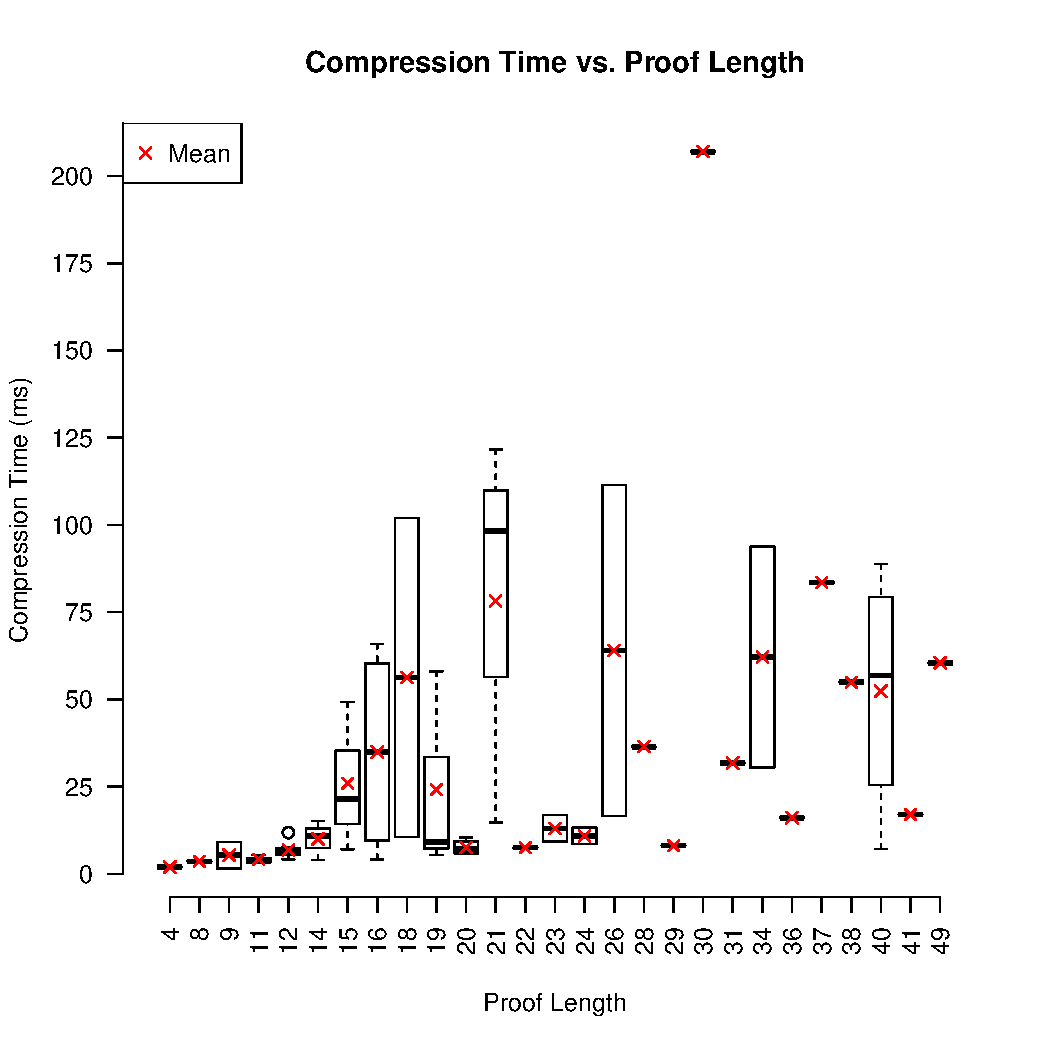
\includegraphics[scale=0.5]{images/compress_time_vs_proof_length.pdf}
\end{figure}

\begin{figure}
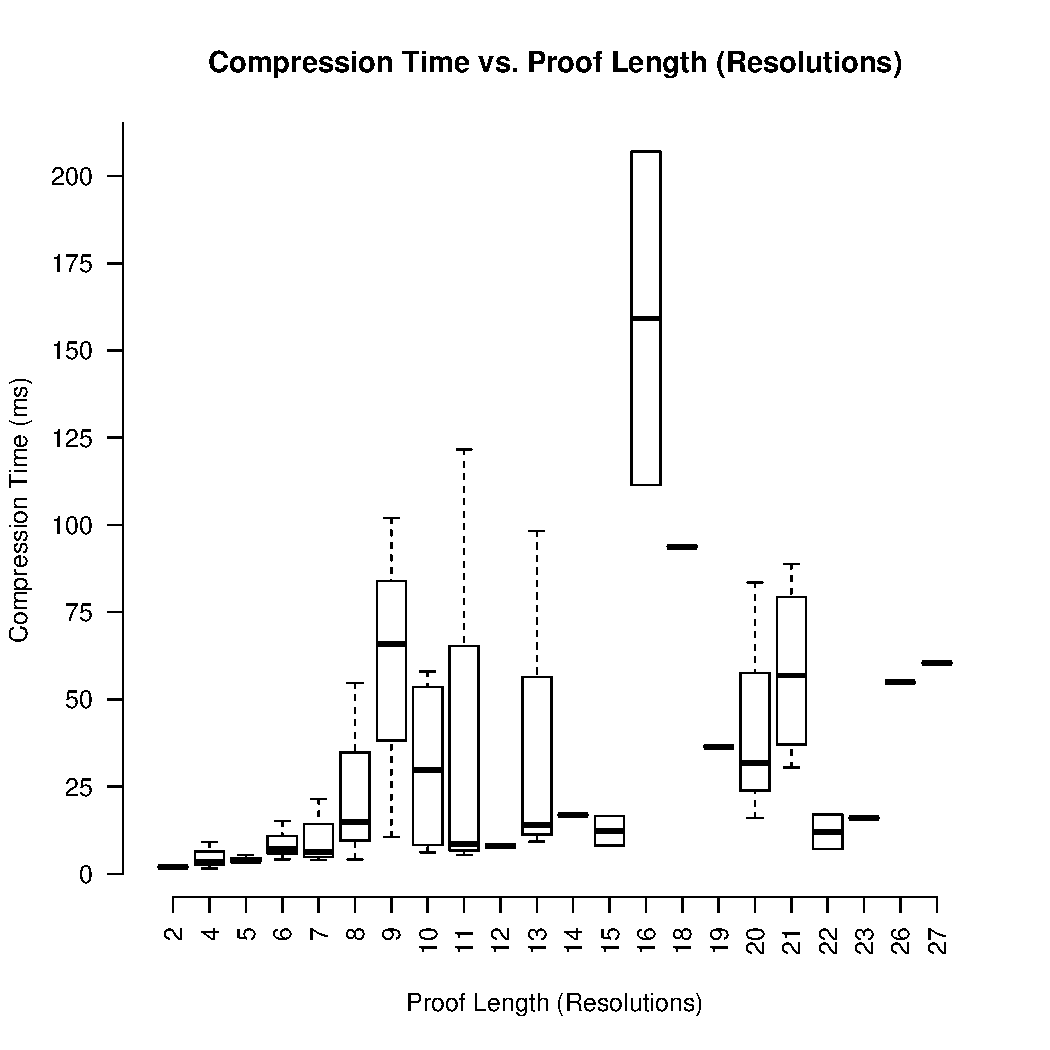
\includegraphics[scale=0.5]{images/compress_time_vs_proof_length_res.pdf}
\end{figure}

\begin{figure}
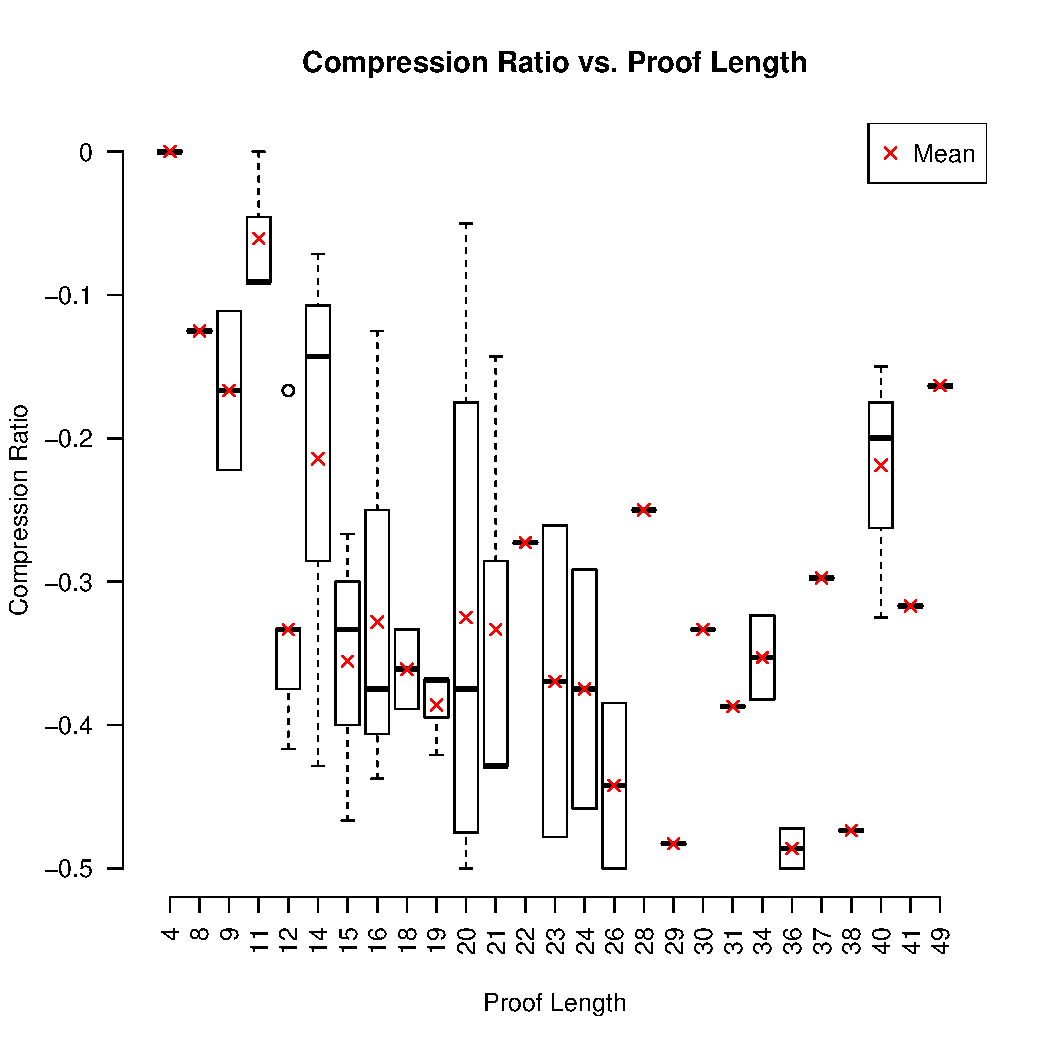
\includegraphics[scale=0.5]{images/compress_ratio_vs_proof_length.pdf}
\end{figure}

\begin{figure}
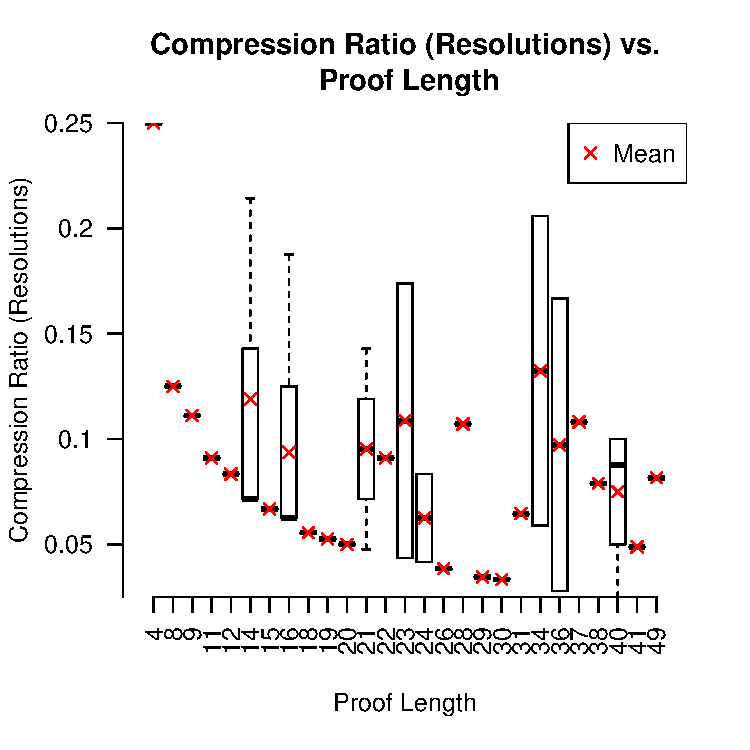
\includegraphics[scale=0.5]{images/compress_ratio_res_vs_proof_length.pdf}
\end{figure}

\begin{figure}
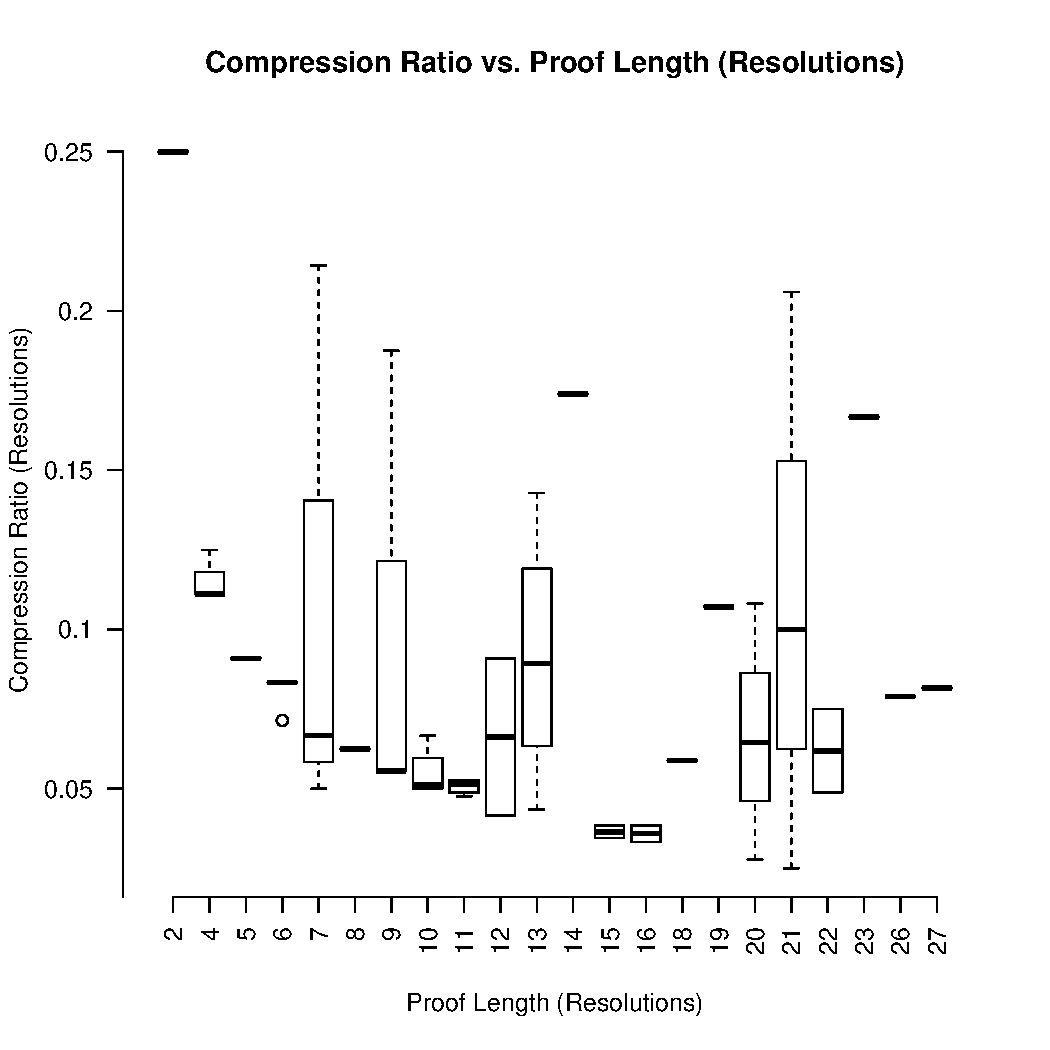
\includegraphics[scale=0.5]{images/compress_ratio_res_vs_proof_length_res.pdf}
\end{figure}

\begin{figure}
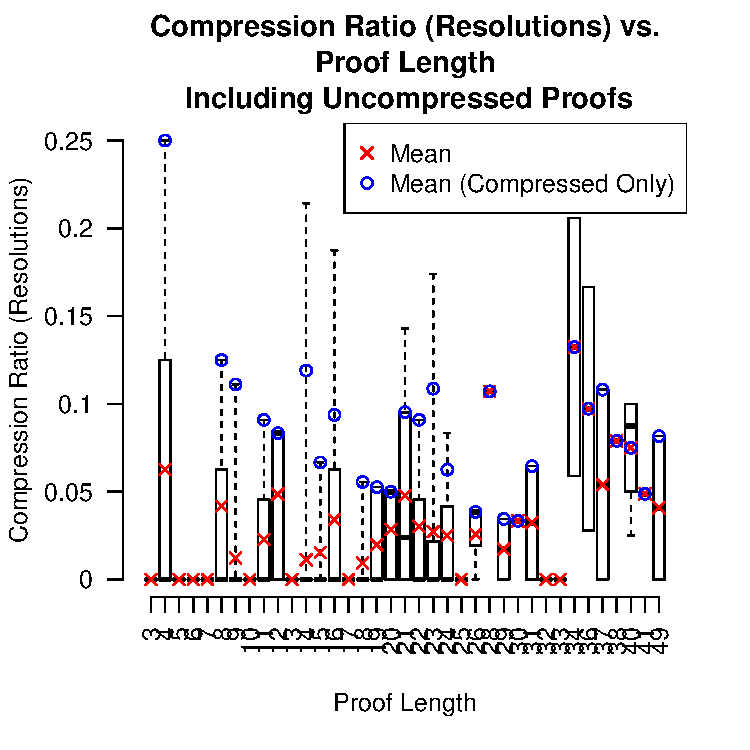
\includegraphics[scale=0.5]{images/compress_ratio_res_vs_proof_length_all_proofs.pdf}
\end{figure}

\begin{figure}
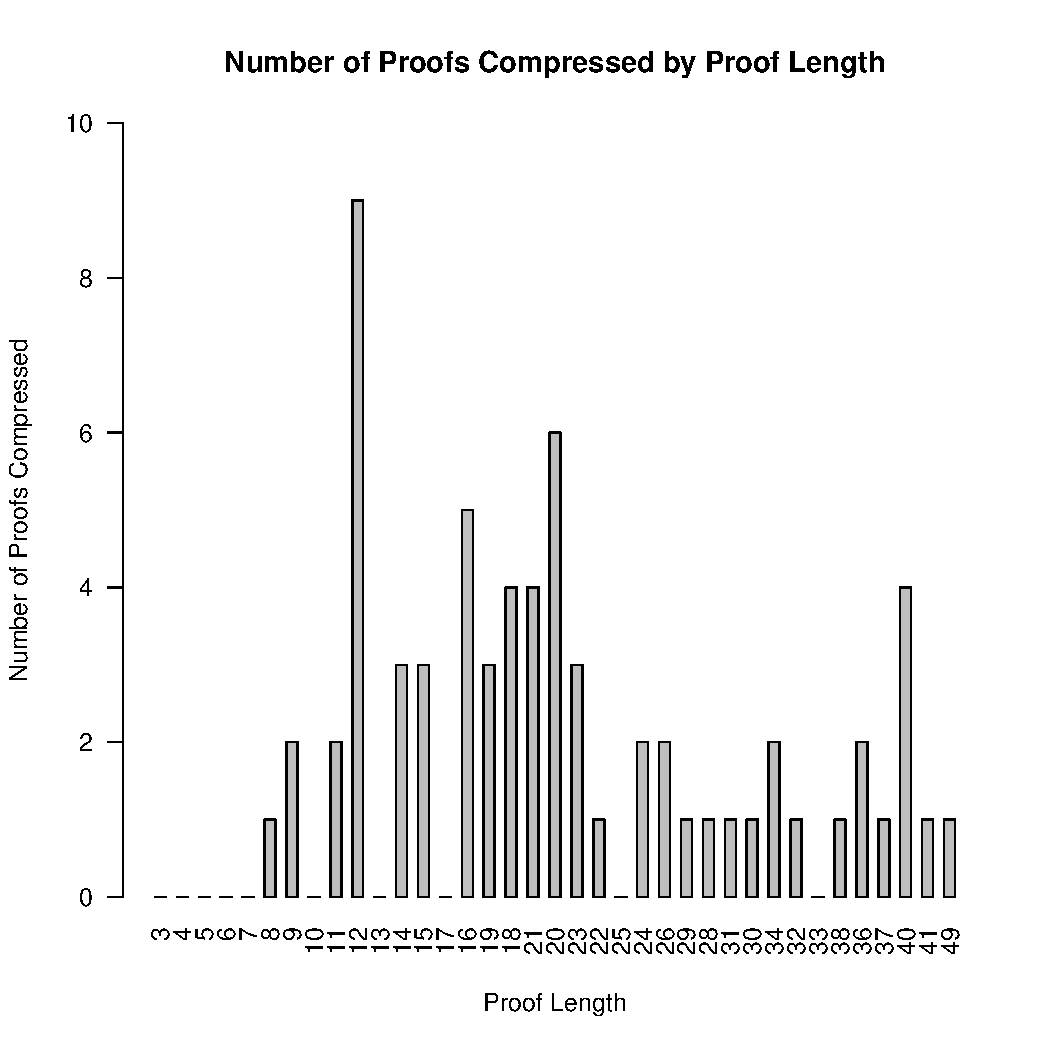
\includegraphics[scale=0.5]{images/num_compressed_count.pdf}
\end{figure}
\begin{figure}
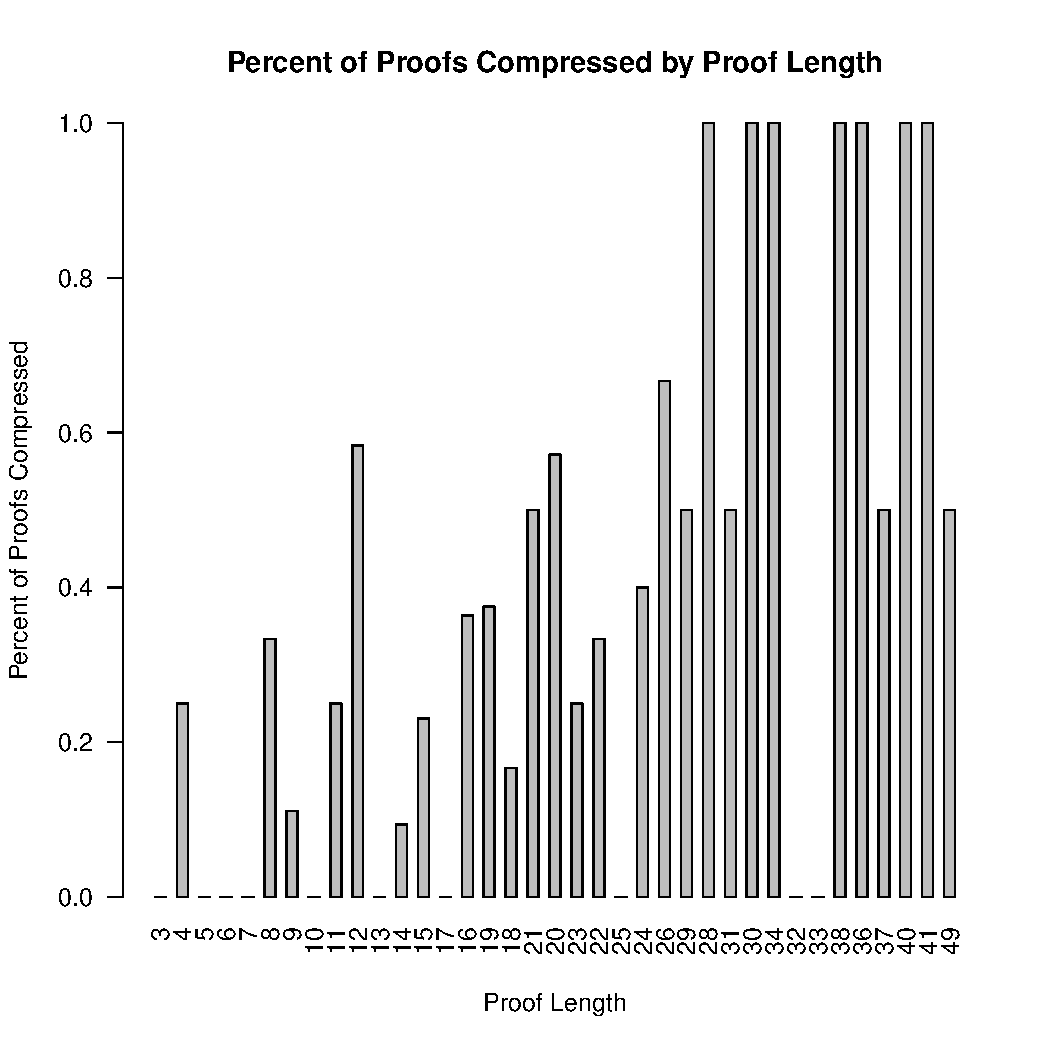
\includegraphics[scale=0.5]{images/num_compressed_percent.pdf}
\end{figure}
\begin{figure}
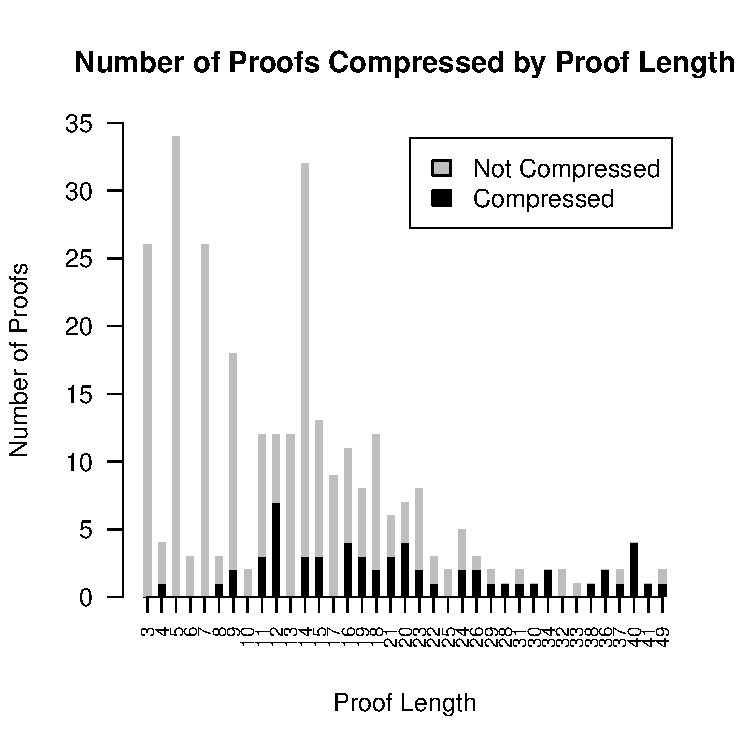
\includegraphics[scale=0.5]{images/num_compressed_stacked.pdf}
\end{figure}

\begin{figure}
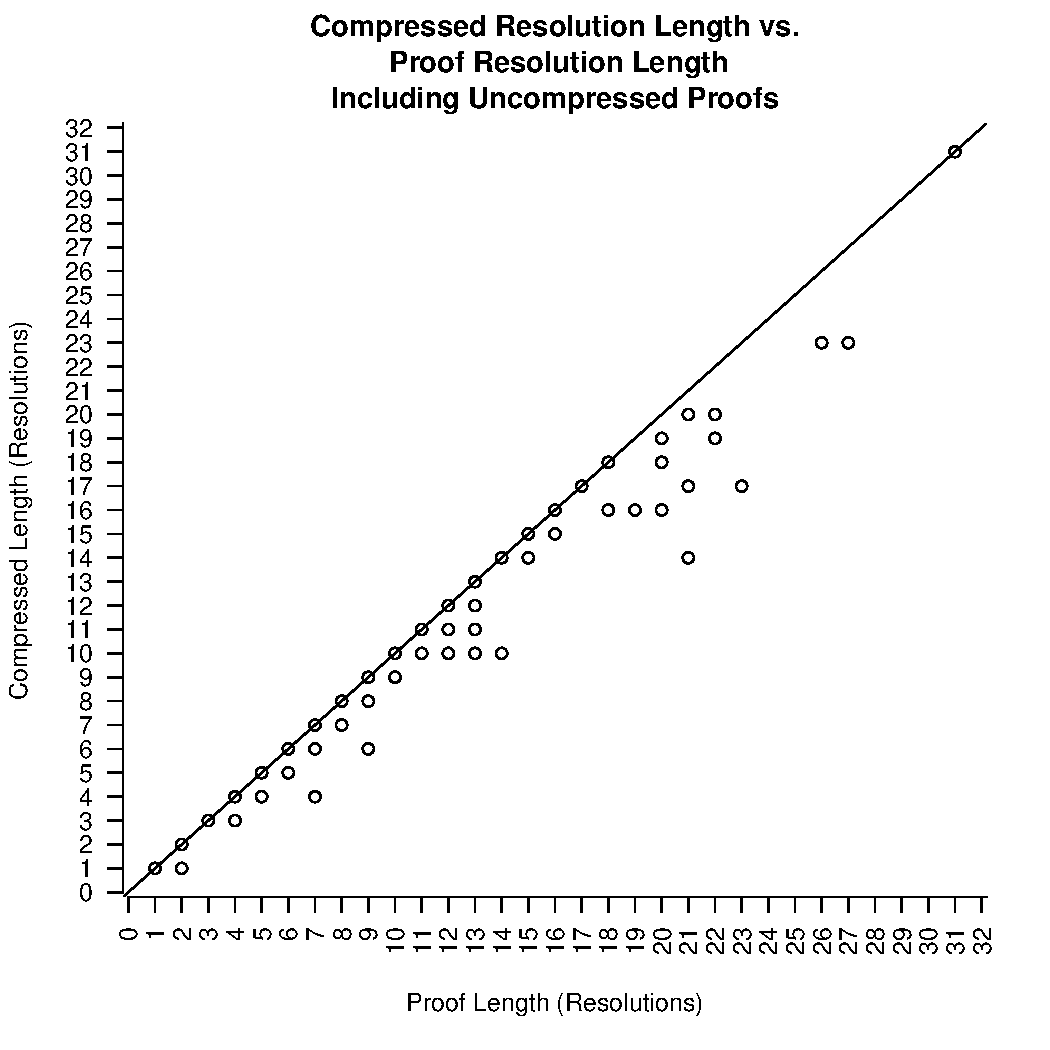
\includegraphics[scale=0.5]{images/res_length_vs_compress_res_length_all_proofs.pdf}
\end{figure}
\begin{figure}
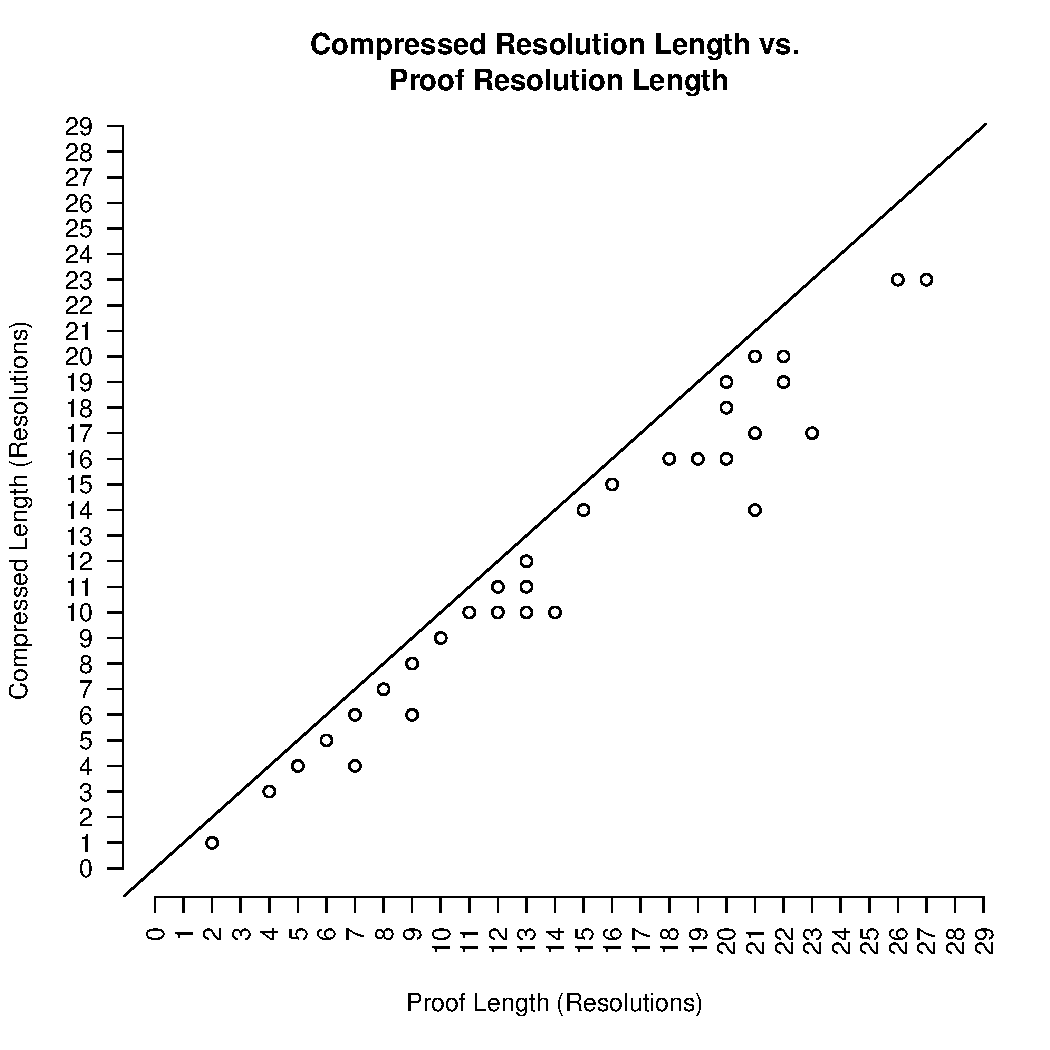
\includegraphics[scale=0.5]{images/res_length_vs_compress_res_length.pdf}
\end{figure}

\begin{figure}
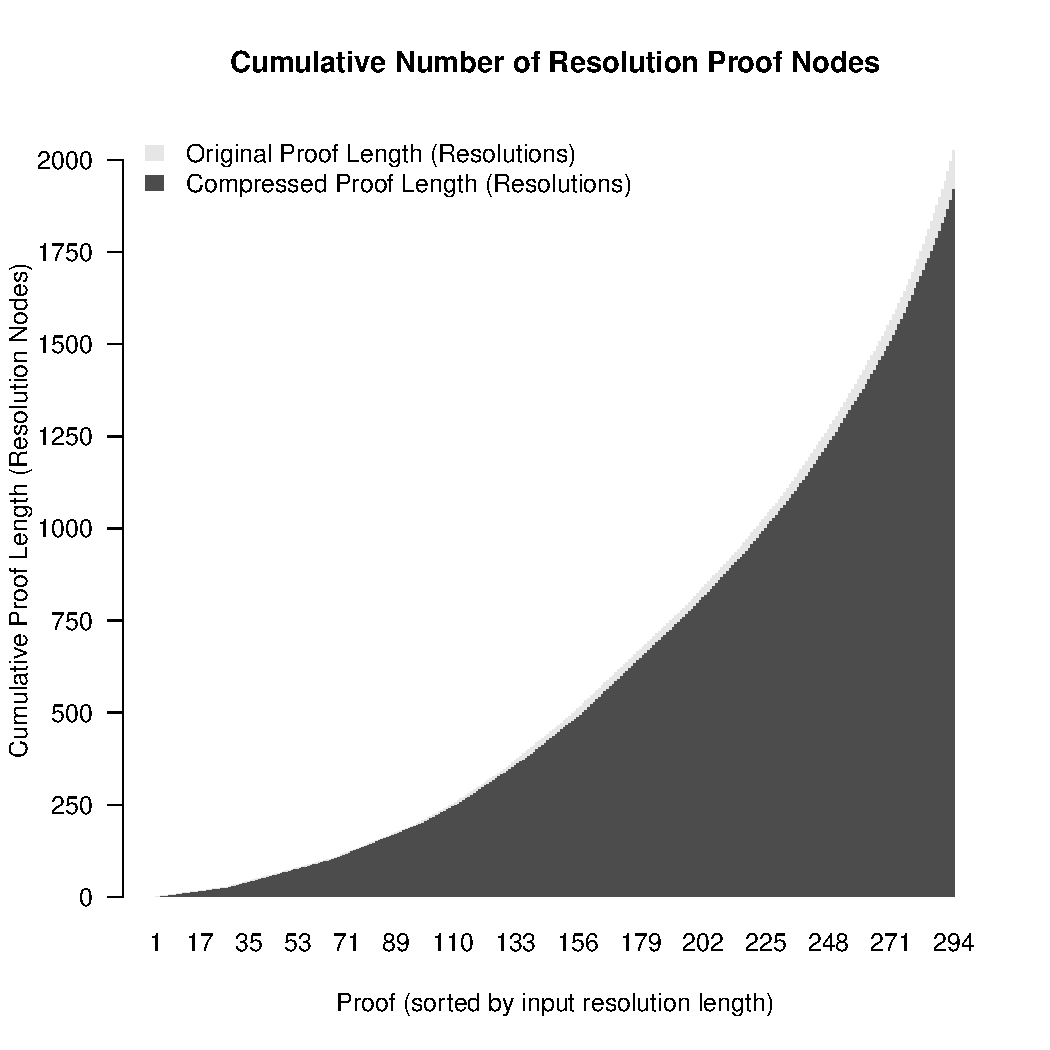
\includegraphics[scale=0.5]{images/cumulative_res_nodes.pdf}
\end{figure}

\begin{figure}
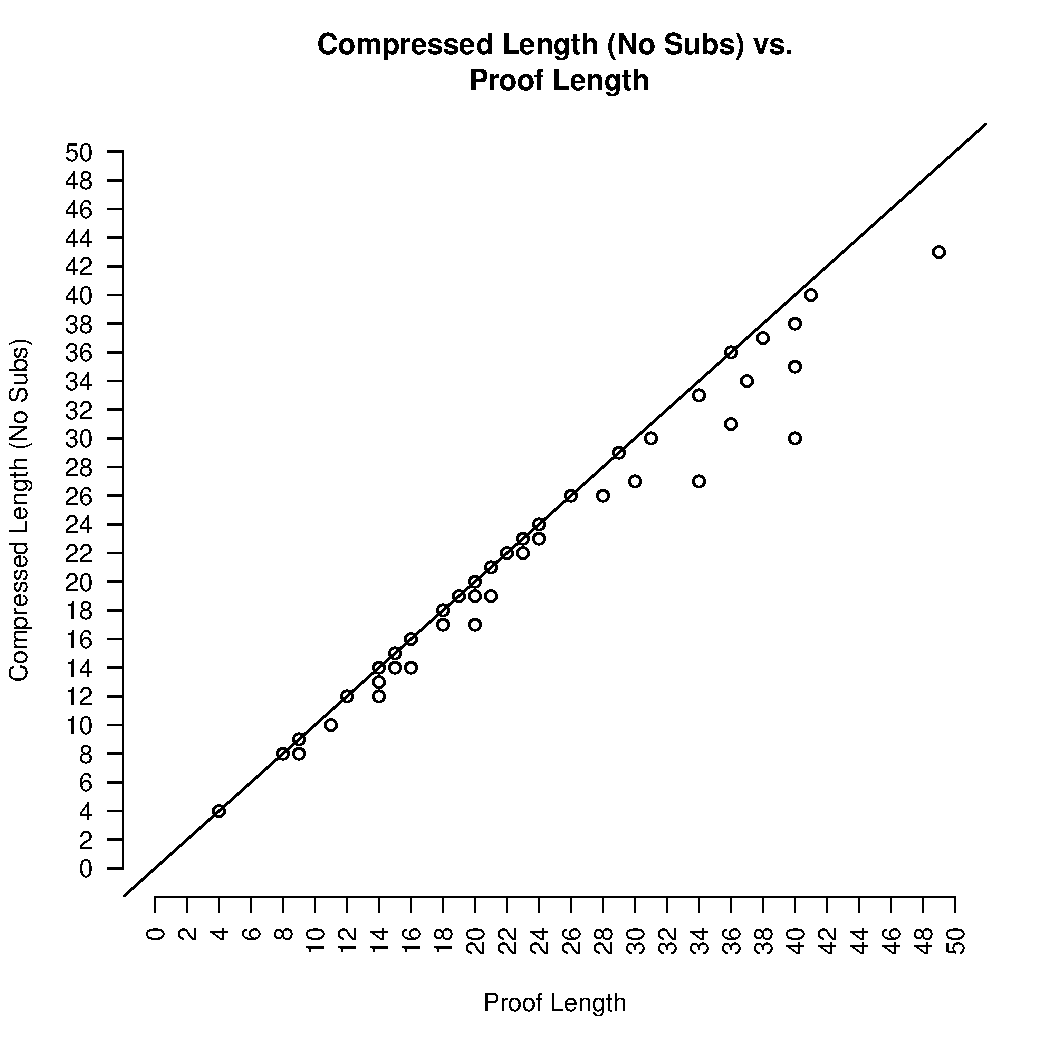
\includegraphics[scale=0.5]{images/compress_length_no_sub_vs_length.pdf}
\end{figure}
\begin{figure}
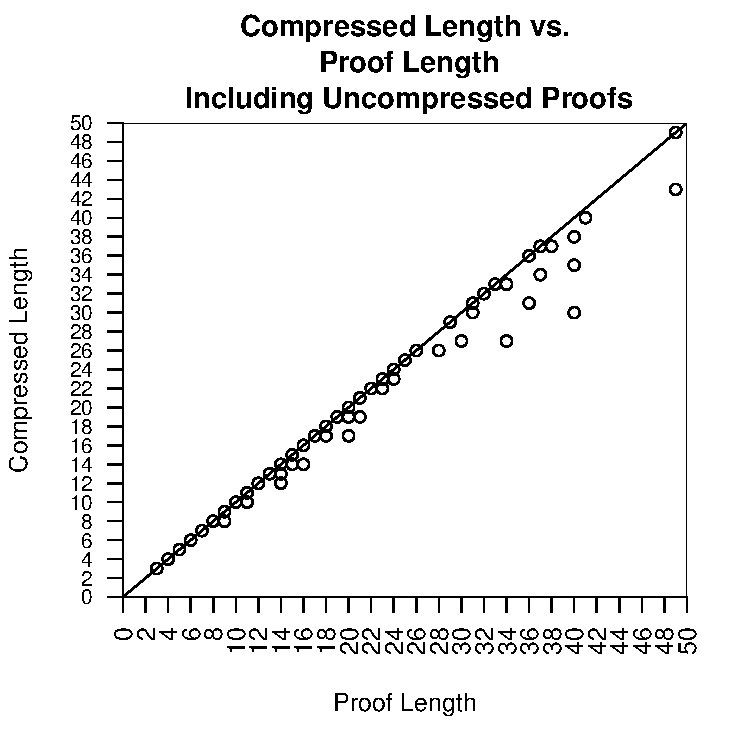
\includegraphics[scale=0.5]{images/compress_length_no_sub_vs_length_all_proofs.pdf}
\end{figure}